\section{allg Problemstellung}
Im folgen werde ich zunächst den Algorithmus aus dem Paper beschreiben und erklären, sowie im Anschluss ein paar Modifikationen, mit denen ich in dieser Bachelorarbeit weiterarbeiten werde.



\subsection{orginaler Algo}
Um die Anzahl der Agenten zu ermitteln, schicken sich die Baumknoten gegenseitig Nachrichten, mit der Information, wie viele Agenten mindestens benötigt werden, um einen bestimmten Teilbaum zu dekontaminieren.
\\
Als erstes berechnet der Algorithmus alle von allen Knoten ihre Knotengewichte. Dieses ergibt sich jeweils aus dem maximalen Kantengewicht aller zu diesem Knoten führenden Kanten. Also für das Knotengewicht vom Knoten x gilt: $\omega(x) = max_{e} \omega(e)$, für jede Kante e inzident zu x.
\\
\\
Nun werden die Nachrichten versendet, für die es zwei Fälle gibt:

\begin{enumerate}
		
	
	\item Fall:
	
		\begin{minipage}{0.55\textwidth} 
			Der aktuelle Knoten x hat bereits schon mindestens n-1 Nachrichten erhalten, wobei n die Anzahl der inzidenten Knoten ist.\\
			
			Um eine Nachricht an den Nachbarknoten y zu senden, nimmt man die 2 größten Nachrichten die bei x angekommen sind (die Nachricht von y wird ignoriert!). Mit diesen beiden angekommenen Nachrichten $l_{1} \ge l_{2}$ sowie dem Knotengewicht $\omega(x)$ wird die Nachricht $\lambda_{y}$ an y wie folgt berechnet:\\
			$\lambda_{y} = max\{l_{1},  l_{2} + \omega(x)\}$
		\end{minipage}
		\hfill
		\begin{minipage}{0.35\textwidth}
			
			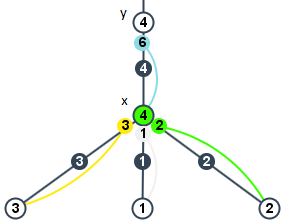
\includegraphics[width=\textwidth]{bilder/abb_paper_n-1knoten.png}
			\captionof{figure}{Die neue Nachricht (blau) von Knoten x zu Knoten y ist 6, da $l_{2} + \omega(x)$ (grün) größer ist als $l_{1}$ (gelb).}
		\end{minipage}

		
		
	\item Fall:
		
		\begin{minipage}{0.55\textwidth} 
			Zu beginn des Algorithmus, oder wenn der andere Fall nicht mehr auftritt, sendet ein beliebiger Blattknoten seine Nachricht an den eigenen Nachbarn.\\
			
			Die zu sendende Nachricht $\lambda_{y}$ vom Blatt x an seinen Nachbarknoten y ist dabei nur das eigene Gewicht:\\
			$\lambda_{y} = \omega(x)$
		\end{minipage}
		\hfill
		\begin{minipage}{0.35\textwidth}
						
			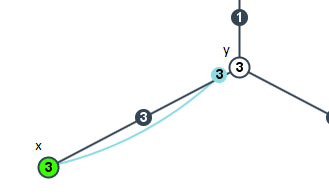
\includegraphics[width=\textwidth]{bilder/abb_blattknoten.png}
			\captionof{figure}{Das Knotengewicht des Blattknotens x (grün) bestimmt die Nachricht (blau) zum Nachbarknoten y.}
		\end{minipage}
		

\end{enumerate}


\subsection{neue interpreatation}
//wieso?

		fzw aegf wfgeewg fzw aegf wfgeewg fzw aegf wfgeewg fzw aegf wfgeewg fzw aegf wfgeewg fzw aegf wfgeewg fzw aegf wfgeewg fzw aegf wfgeewg fzw aegf wfgeewg fzw aegf wfgeewg fzw aegf wfgeewg fzw aegf wfgeewg fzw aegf wfgeewg fzw aegf wfgeewg fzw aegf wfgeewg fzw aegf wfgeewg fzw aegf wfgeewg fzw aegf wfgeewg fzw aegf wfgeewg fzw aegf wfgeewg fzw aegf wfgeewg fzw aegf wfgeewg fzw aegf wfgeewg fzw aegf wfgeewg fzw aegf wfgeewg fzw aegf wfgeewg fzw aegf wfgeewg fzw aegf wfgeewg fzw aegf wfgeewg fzw aegf wfgeewg fzw aegf wfgeewg fzw aegf wfgeewg fzw aegf wfgeewg fzw aegf wfgeewg fzw aegf wfgeewg fzw aegf wfgeewg fzw aegf wfgeewg fzw aegf wfgeewg fzw aegf wfgeewg fzw aegf wfgeewg fzw aegf wfgeewg fzw aegf wfgeewg fzw aegf wfgeewg fzw aegf wfgeewg 


		\begin{wrapfigure}{r}{0.5\textwidth}
			\begin{center}
				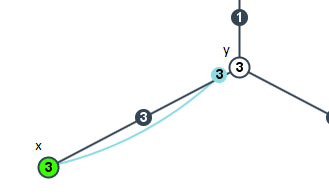
\includegraphics[width=0.48\textwidth]{bilder/abb_blattknoten.png}
			\end{center}
			\caption{A gull}
		\end{wrapfigure}
		
		
		
		
		
		fzw aegf wfgeewg fzw aegf wfgeewg fzw aegf wfgeewg fzw aegf wfgeewg fzw aegf wfgeewg fzw aegf wfgeewg fzw aegf wfgeewg fzw aegf wfgeewg fzw aegf wfgeewg fzw aegf wfgeewg fzw aegf wfgeewg fzw aegf wfgeewg fzw aegf wfgeewg fzw aegf wfgeewg fzw aegf wfgeewg fzw aegf wfgeewg fzw aegf wfgeewg fzw aegf wfgeewg fzw aegf wfgeewg fzw aegf wfgeewg fzw aegf wfgeewg fzw aegf wfgeewg fzw aegf wfgeewg fzw aegf wfgeewg fzw aegf wfgeewg fzw aegf wfgeewg fzw aegf wfgeewg fzw aegf wfgeewg fzw aegf wfgeewg fzw aegf wfgeewg fzw aegf wfgeewg fzw aegf wfgeewg wfgeewg fzw aegf wfgeewg fzw aegf wfgeewg fzw aegf wfgeewg fzw aegf wfgeewg fzw aegf wfgeewg fzw aegf wfgeewg fzw aegf wfgeewg fzw aegf wfgeewg fzw aegf wfgeewg fzw aegf wfgeewg fzw aegf wfgeewg fzw aegf wfgeewg fzwfgeewg fzw aegf wfgeewg fzw aegf wfgeewg fzw aegf wfgeewg fzw aegf wfgeewg fzw aegf wfgeewg fzw aegf wfgeewg fzw aegf wfgeewg fzw aegf wfgeewg fzw aegf wfgeewg fzw aegf wfgeewg fzw aegf wfgeewg fzw aegf wfgeewg fzwfgeewg fzw aegf wfgeewg fzw aegf wfgeewg fzw aegf wfgeewg fzw aegf wfgeewg fzw aegf wfgeewg fzw aegf wfgeewg fzw aegf wfgeewg fzw aegf wfgeewg fzw aegf wfgeewg fzw aegf wfgeewg fzw aegf wfgeewg fzw aegf wfgeewg fzwfgeewg fzw aegf wfgeewg fzw aegf wfgeewg fzw aegf wfgeewg fzw aegf wfgeewg fzw aegf wfgeewg fzw aegf wfgeewg fzw aegf wfgeewg fzw aegf wfgeewg fzw aegf wfgeewg fzw aegf wfgeewg fzw aegf wfgeewg fzw aegf wfgeewg fz

		
	